\articlehead{The Furry Accommodation Network}{JM}{2012}

The furry community is expanding worldwide. Here on [adjective][species], Zik has been chronicling all things international with his comprehensive survey of conventions outside of North America -- Furry Cons of the World -- and his insight into the growing Japanese community -- Foreign Furry Fandoms: Japan. Both articles are required reading for anyone wanting evidence of furry's global growth. I understand that there is more to come from Zik, who is rapidly becoming the go-to chronicler of internationalism in our community.

One of the frontiers of the furry community is South-East Asia, with the local furry group -- AnthroAsia -- loosely incorporating Singapore, Malaysia, Thailand, Indonesia, and the Philippines. The group maintains an internet presence at www.anthroasia.com, which includes a fairly quiet forum with just over 400 registered members. The forums are quiet because most of the local furry chatter happens on Facebook, however the AA forums are heavily lurked and are therefore a great place for new furries to introduce themselves.

I recently visited Malaysia and wondered whether a local furry or two might be available to catch up during my stay. I'd met a few of the AA crew before, all Singaporeans, and guessed that they might know someone. I made the laziest possible attempt to make contact: a single tweet.

\begin{figure}
  \begin{center}
    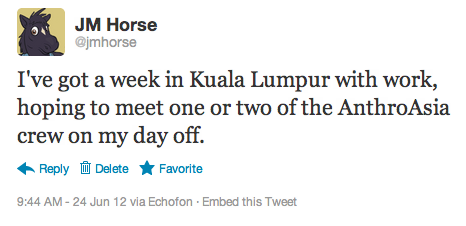
\includegraphics{content/assets/furry-accommodation--jmtweet}
  \end{center}
  \caption{Casting out}
\end{figure}

What happened next was predictable and simple and magical: a Singaporean furry saw my tweet and left a one-line public `shout' at AnthroAsia.com; a Malaysian furry saw the note and got in contact. Shortly afterwards, I found myself with a furry in a mamak -- a 24-hour open-air food market -- at 2am on the outskirts of Kuala Lumpur. My host, Hiro Husky, had decided that a night-time meal would be perfect given my jetlag.

The food and environment were new to me, and I'd never met Hiro before, but the fellowship and friendly connection was as comfortable and familiar as my favourite stuffed zebra. Amongst furries, there is an implied trust and closeness. It's never more evident than when you experience it with a stranger in an unfamiliar place.

Long-distance travel is central to the furry experience. For many furries, a trip to their first big convention is a pilgrimage of sorts: an important step in community engagement as they explore a large gathering for the first time. For those lucky enough to have experienced it, it's great standing at a check-in queue and scanning the crowd for discreet collars, or bags big enough to carry a fursuit, or people wearing slightly tragic wolf-howling-at-the-moon t-shirts.

Outside of trips to conventions, furries fly around the world for more modest events: meeting an online romantic partner for the first time, visiting old friends, or meeting new furries in a new location as a tourist.

Long-distance travel is especially important to us because so much of the furry experience takes place on the internet, which means we're less restricted by distance's tyranny. With friends around the world, we're more likely to get passports and catch planes or trains than our non-furry peers.

When you first meet a new furry in real life, there is an implicit level of trust. I think this is because of our common reliance on the community, a community that reinforces of our internal self-image, a club where the only requirement for membership is to decide you're a member. We're trusting because of our fellowship within the community: everyone wants to make a good impression.

The implied promise of trust and mutual respect means that furries are often willing to offer a visitor a place to sleep, perhaps a couch or a spare bed. Over the years I have offered a roof to dozens of furries, and have accepted as many offers when I have been travelling. I like to call this the Furry Accommodation Network.

To offer accommodation is a selfless act, but one that's paid back by the generosity of the community at large. Far more than an ad hoc couch-surfing network, staying with furries offers immediate company, probable friendship and -- sometimes -- the genesis of a relationship.

It's not all roses of course. I have had some bad experiences, both when travelling and when hosting, however these have all aged into amusing anecdotes. The friendships I have formed or reinforced through such arrangements remain strong and continue to grow today.

I stayed in a hotel in Kuala Lumpur but the advantages of the Furry Accommodation Network were all there, thanks to Hiro's selflessness and generosity. I experienced a side of KL I could never have found as a mere tourist and I got to know a remarkable furry in Hiro.

Our conversation at the mamak started with furry and quickly spread to mutual passions: food, sex, and politics. Over flatbreads and dal soup, Hiro asked me about my relationship and the freedoms I enjoy as part of a gay couple in London. I responded that it's pretty good, and improving -- that gay marriage isn't legal but it's on the way; that my partner and I can act as openly as a straight couple in much of the city; that I am openly gay amongst my friends and colleagues, and that anyone with a problem would be considered a bigot.

Hiro counterpointed this with his experience in Malaysia. If he were to express physical affection towards his boyfriend then he could find himself arrested and tried under Sharia law. (Sharia law technically only applies to Muslims in Malaysia -- Hiro is of Chinese background -- but a homosexuality case could be considered to be a Sharia `issue'). Change in Malaysia is unlikely because there are laws in place that limit the ability for people to criticise the government, and the same party has been in power since Independence. Hiro is closeted amongst everyone outside of furry.

This is not to say that homosexuality doesn't exist in Malaysia. Hiro and I were shopping in the geek heaven that is Plaza Low Yat, a seven-level shopping mall dedicated to all things IT. On two separate occasions, Hiro was given overt come-ons by guys as we walked past. Hiro is an attractive guy but he's not effeminate or otherwise sending out gay vibes in any way that I noticed, so these couldn't have been one-off incidents. I think that Hiro tries to maintain an asexual mask when out in public, and he was apparently oblivious in both cases. Suffice to say that a gay person, if they were so inclined, would still be able to meet people in KL.

When we were chatting, I talked about how fortunate I feel to be a part of the furry community. We both share the common experience of being blown away by the mere existence of furries. Furry has also helped our personal growth -- Hiro and I are both included amongst those who re-evaluated their sexual preference after joining the community. On reflection, Hiro is probably more fortunate than me to have found furry: furry is the only environment where he can be an honest version of himself.

This is mostly a product of the illiberal Malaysian culture, which is comparable to most of the countries in the region. Things are better in Singapore -- Hiro visits regularly -- but it's still much less permissive than countries like the UK.

For the AnthroAsia furries, participation in the furry group is very valuable. This is especially true for those furries with an unusual sexual orientation, gender identity or self-image. The AA group has grown quickly since its formal inception, and seems very likely to continue its growth as it is discovered by more young furries who might be lacking a rewarding social experience in mainstream circles.

My experience of getting to know Hiro and comparing our respective furry experiences reinforced what I think is great about our community. The Furry Accommodation Network -- with its implied trust and mutual respect -- is a microcosm of the happiness and self-realization that furry can bring.

Later this year, Hiro is travelling to Eurofurence with a few fellow AnthroAsia furries. It'll be the first time he's travelled outside of Malaysia or Singapore. He's nervous about being around a large group, unsure of social norms in Germany, and concerned about language barriers. And he's excited to experience his first pilgrimage to a large convention.

The feeling of excitement is mutual.

\begin{figure}
  \begin{center}
    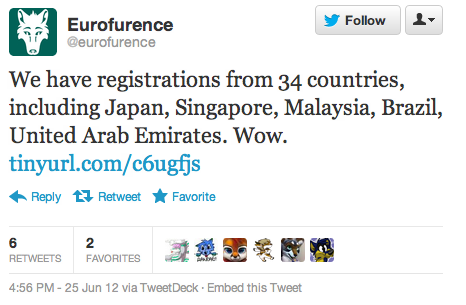
\includegraphics{content/assets/furry-accommodation--eftweet}
  \end{center}
  \caption{Eurofurence stats}
\end{figure}

He'll have a great time.
